\subsection{2021年1月4日}
\paragraph{\href{https://www.51voa.com/VOA\_Special\_English/scientists-declare-climate-emergency-83245.html}{原文}}

\begin{figure}[H]
\centering
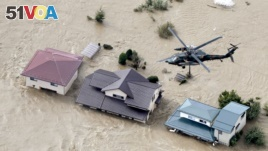
\includegraphics[scale=0.7]{002_voa_20210104.jpg}
\caption{An aerial view shows a Japan Self-Defence Force helicopter flying over residential areas flooded by the Chikuma river following Typhoon Hagibis in Nagano, central Japan, October 13, 2019, in this photo taken by Kyodo.}
\end{figure}

%\begin{messagebox}
By Jonathan Evans
09 November, 2019
More than 11,000 scientists are warning that the Earth, in their words, "clearly and unequivocally faces a climate emergency."
The scientists represent several fields of study and come from 150 countries around the world. They approved a report that appeared in the publication Bioscience earlier this month. It warns that the world would face "untold human suffering" if it does not make deep and lasting shifts in human activities that influence climate change.
The new report is called the "World Scientists' Warning of a Climate Emergency." Three leaders of the study are from the United States. They are ecologists Bill Ripple and Christopher Wolf of Oregon State University and William Moomaw of Tufts University in Massachusetts. The three worked on the study with scientists from universities in South Africa and Australia.
This is the first time a large group of scientists have jointly used the word "emergency" when talking about climate change.
"Despite 40 years of global climate negotiations...we have generally conducted business as usual and have largely failed to address this predicament," the study said. "Climate change has arrived and is accelerating faster than many scientists expected."
The report identified six areas that the world needs to deal with immediately. The scientists appealed to nations to use energy more efficiently and cut their use of fossil fuels. They suggested that lawmakers approve taxes on the burning of carbon-based fuels, such as coal, oil and natural gas.
The scientists expressed support for women's rights and making family planning services "available to all people." They said this would help to reduce sudden or unexpected changes in the size of the human population.
The report urges people to move toward more of a plant-based diet.
Other areas of concern include preventing the destruction of forests and permanent loss of some plant and animal species.
The reported noted that it will most likely take strong actions by the public to move politicians to approve lasting policy changes.
The scientists added, "We believe that the prospects will be greatest if decision-makers and all of humanity promptly respond to this warning and declaration of a climate emergency, and act to sustain life on planet Earth, our only home."
I'm Jonathan Evans.
VOANews.com reported this story. Jonathan Evans adapted the story for Learning English. George Grow was the editor.
%\end{messagebox}

\begin{messagebox}
Words in This Story
accelerating – adj. increasing in speed or rate of occurrence
address – v. to deal with; give attention to
fossil fuels – n. fuels such as coal, oil, or natural gas that formed in the earth from dead plants or animals
predicament – n. a difficult or unpleasant situation
prospects – n. opportunities for something to happen
shifts – n. changes in how something is done or how people think about something
sustain – v. to provide what is needed for something or someone to exist, continue, etc.
unequivocally – adv. in an unequivocal manner
\end{messagebox}

%\begin{messagebox}
More than 11,000 scientists are warning that the Earth, in their words, "clearly and unequivocally faces a climate emergency."
超过11000名科学家发出了警告,用他们的话来说是,地球“显然并且毫无疑问地遇到了气候紧急状况。”
The scientists represent several fields of study and come from 150 countries around the world. They approved a report that appeared in the publication Bioscience earlier this month. It warns that the world would face "untold human suffering" if it does not make deep and lasting shifts in human activities that influence climate change.
来自全球150个国家的这些科学家们代表了多个研究领域。他们通过的一份报告发表在本月初的《生物科学》杂志上。这份报告警告称,如果不对影响气候变化的人类活动作出深刻而持久的改变,世界将面临“巨大的人类苦难。”
The new report is called the "World Scientists' Warning of a Climate Emergency." Three leaders of the study are from the United States. They are ecologists Bill Ripple and Christopher Wolf of Oregon State University and William Moomaw of Tufts University in Massachusetts. The three worked on the study with scientists from universities in South Africa and Australia.
这份新报告名为《全球科学家对气候紧急状况发出的警告》。该研究的三位领导者来自美国。他们是俄勒冈州里大学的生态学家比尔·瑞博和克里斯托弗·沃尔夫,以及马萨诸塞州塔夫茨大学的威廉·穆茂。这三人与来自南非和澳大利亚各大学的科学家们一起进行了这项研究。
This is the first time a large group of scientists have jointly used the word "emergency" when talking about climate change.
这是首次有一大批科学家在谈到气候变化时共同使用了“紧急状况”这个词。
"Despite 40 years of global climate negotiations...we have generally conducted business as usual and have largely failed to address this predicament," the study said. "Climate change has arrived and is accelerating faster than many scientists expected."
研究称:“尽管全球气候谈判已经进行了40年,但我们一直照常开展业务,并且在很大程度上未能解决这一困境。气候变化已经到来,并且其加速度超过了许多科学家的预期。”
The report identified six areas that the world needs to deal with immediately. The scientists appealed to nations to use energy more efficiently and cut their use of fossil fuels. They suggested that lawmakers approve taxes on the burning of carbon-based fuels, such as coal, oil and natural gas.
这份报告确立了全球需要立即处理的6大领域。科学家们呼吁各国更加有效地利用能源并减少化石燃料的使用。他们建议立法者批准对燃烧煤炭、石油和天然气等碳基燃料征税。
The scientists expressed support for women's rights and making family planning services "available to all people." They said this would help to reduce sudden or unexpected changes in the size of the human population.
科学家们表示支持妇女权利,并使计划生育服务“向所有人提供。”他们表示,这将会有助于减少人口规模突然或意外发生变化。
The report urges people to move toward more of a plant-based diet.
报告督促人们朝着以植物性饮食为主的方向发展。
Other areas of concern include preventing the destruction of forests and permanent loss of some plant and animal species.
其它令人关注的领域包括防止森林遭到破坏,以及防止某些动植物物种遭受永久性损失。
The reported noted that it will most likely take strong actions by the public to move politicians to approve lasting policy changes.
报告指出,公众很可能会采取强有力的行动,督促政客批准可持续的政策改革。
The scientists added, "We believe that the prospects will be greatest if decision-makers and all of humanity promptly respond to this warning and declaration of a climate emergency, and act to sustain life on planet Earth, our only home."
这些科学家们还说:“我们相信,如果决策者和全人类迅速响应这一警告并宣布气候紧急状态,采取行动维护地球这个我们唯一家园的生命,那么就会有伟大的前景。”
%\end{messagebox}
